%%%%%%%% ICML 2025 EXAMPLE LATEX SUBMISSION FILE %%%%%%%%%%%%%%%%%

\documentclass{article}

% Recommended, but optional, packages for figures and better typesetting:
\usepackage{microtype}
\usepackage{graphicx}
\usepackage{subfigure}
\usepackage{booktabs} % for professional tables
\usepackage{multirow}

% hyperref makes hyperlinks in the resulting PDF.
% If your build breaks (sometimes temporarily if a hyperlink spans a page)
% please comment out the following usepackage line and replace
% \usepackage{icml2025} with \usepackage[nohyperref]{icml2025} above.
\usepackage{hyperref}


% Attempt to make hyperref and algorithmic work together better:
\newcommand{\theHalgorithm}{\arabic{algorithm}}

% Use the following line for the initial blind version submitted for review:
\usepackage{icml2025}

% If accepted, instead use the following line for the camera-ready submission:
% \usepackage[accepted]{icml2025}

% For theorems and such
\usepackage{amsmath}
\usepackage{amssymb}
\usepackage{mathtools}
\usepackage{amsthm}
\usepackage{tikz}
\usetikzlibrary{positioning,calc}

% if you use cleveref..
\usepackage[capitalize,noabbrev]{cleveref}

%%%%%%%%%%%%%%%%%%%%%%%%%%%%%%%%
% THEOREMS
%%%%%%%%%%%%%%%%%%%%%%%%%%%%%%%%
\theoremstyle{plain}
\newtheorem{theorem}{Theorem}[section]
\newtheorem{proposition}[theorem]{Proposition}
\newtheorem{lemma}[theorem]{Lemma}
\newtheorem{corollary}[theorem]{Corollary}
\theoremstyle{definition}
\newtheorem{definition}[theorem]{Definition}
\newtheorem{assumption}[theorem]{Assumption}
\theoremstyle{remark}
\newtheorem{remark}[theorem]{Remark}

% Todonotes is useful during development; simply uncomment the next line
%    and comment out the line below the next line to turn off comments
%\usepackage[disable,textsize=tiny]{todonotes}
\usepackage[textsize=tiny]{todonotes}


% The \icmltitle you define below is probably too long as a header.
% Therefore, a short form for the running title is supplied here:
\icmltitlerunning{Compiler Optimizations for Higher-Order Automatic Differentiation in JAX}

\begin{document}

\twocolumn[
\icmltitle{Compiler Optimizations for Higher-Order Automatic Differentiation in JAX}

% It is OKAY to include author information, even for blind
% submissions: the style file will automatically remove it for you
% unless you've provided the [accepted] option to the icml2025
% package.

% List of affiliations: The first argument should be a (short)
% identifier you will use later to specify author affiliations
% Academic affiliations should list Department, University, City, Region, Country
% Industry affiliations should list Company, City, Region, Country

% You can specify symbols, otherwise they are numbered in order.
% Ideally, you should not use this facility. Affiliations will be numbered
% in order of appearance and this is the preferred way.
\icmlsetsymbol{equal}{*}

\begin{icmlauthorlist}
\icmlauthor{Firstname1 Lastname1}{equal,yyy}
\end{icmlauthorlist}

\icmlaffiliation{yyy}{Department of XXX, University of YYY, Location, Country}
\icmlaffiliation{comp}{Company Name, Location, Country}
\icmlaffiliation{sch}{School of ZZZ, Institute of WWW, Location, Country}

\icmlcorrespondingauthor{Firstname1 Lastname1}{first1.last1@xxx.edu}
\icmlcorrespondingauthor{Firstname2 Lastname2}{first2.last2@www.uk}

% You may provide any keywords that you
% find helpful for describing your paper; these are used to populate
% the "keywords" metadata in the PDF but will not be shown in the document
\icmlkeywords{automatic differentiation, compiler optimization, StableHLO, scientific machine learning}

\vskip 0.3in
]

% this must go after the closing bracket ] following \twocolumn[ ...

% This command actually creates the footnote in the first column
% listing the affiliations and the copyright notice.
% The command takes one argument, which is text to display at the start of the footnote.
% The \icmlEqualContribution command is standard text for equal contribution.
% Remove it (just {}) if you do not need this facility.

%\printAffiliationsAndNotice{}  % leave blank if no need to mention equal contribution
\printAffiliationsAndNotice{\icmlEqualContribution} % otherwise use the standard text.

\begin{abstract}
Higher-order automatic differentiation (AD) is increasingly important in
scientific machine learning, but mathematically equivalent methods for computing
Hessians, Hessian-vector products, and Laplacians can lower to substantially
different tensor programs.  We study this effect in JAX by comparing Hessian,
JVP-of-gradient, and Taylor-mode AD formulations, lowering each to StableHLO,
and dispatching both original and transformed programs through XLA.  Our
pipeline combines a direct tanh-MLP Laplacian rewrite with StableHLO constant
propagation and structural-zero elimination.  On MLP Laplacian and Poisson PINN
benchmarks, optimization reduces average runtime by up to \(1.94\times\) and
compile time by up to \(2.28\times\).  The fastest AD method before optimization
is not always the fastest after optimization, suggesting that higher-order AD
method selection should account for downstream compiler optimizability.
\end{abstract}

\section{Introduction}
Automatic differentiation (AD) has become a central tool in machine learning, particuarly in deep learning, enabling the training of complex models in frameworks like PyTorch and TensorFlow. AD computes derivatives by systematically applying the chain rule to the primitive operations of a program, producing derivatives that are exact up to floating-point arithmetic. While most widely used AD systems are optimized for first-order derivatives, many emerging applications require second- and higher-order derivatives, including Hessians, Jacobian-vector products, and Laplacians.

Higher-order AD is expensive, but its cost depends not only on the derivative being computed, but also on how the derivative program is generated and optimized. Different higher-order AD strategies, such as nested first-order AD (e.g. repeatedly applying first-order forward/reverse mode AD) or Taylor-mode AD (e.g. computing higher-order
derivatives via a Taylor series expansion), can produce mathematically equivalent derivatives while lowering to structurally different tensor programs. These differences affect the opportunities available to downstream compiler optimizations.

In this paper, we study higher-order AD as a compiler optimization problem. We lower several higher-order AD methods to StableHLO, apply several optimization passes, and execute both original and optimized programs through XLA. We make the following contributions:

\begin{enumerate}
    \item We present a pipeline for comparing higher-order AD methods before and after compiler optimization.
    \item We evaluate repeated first-order AD compositions and Taylor-mode AD on higher-order derivative workloads.
    \item We show that compiler optimization can substantially improve performance, reducing runtime by up to \(1.94\times\) and compile time by up to \(2.28\times\) on Laplacian benchmarks.
    \item We demonstrate that compiler optimizations can change which AD strategy performs best, suggesting that AD method selection should account for downstream compiler optimizability.
\end{enumerate}

\section{Higher-Order AD Methods Produce Different Compiler IR}

In general, AD constructs a new computation that evaluates derivatives of the original computation. For example, suppose we write a simple JAX function:
\begin{verbatim}
def f(x):
    return x * x + 1.0

g = jax.grad(f)
\end{verbatim}

Mathematically, $g(x)=2x$. However, from the compiler's point of view, \texttt{jax.grad(f)} does not simply record this symbolic formula; instead, it constructs a new program whose operations compute the derivative of \texttt{f}. This distinction becomes especially important for higher-order AD:
two methods may compute the same mathematical derivative while generating
substantially different compiler IR.

In JAX, higher-order derivatives can be computed using transformations such as
\texttt{jax.hessian}, \texttt{jax.jvp}, \texttt{jax.grad}, or \texttt{jax.experimental.jet}. These transformed programs can be traced into JAX's internal \emph{jaxpr}
representation, a functional IR that exposes the primitive operations and data
dependencies of the staged computation. JAX then lowers jaxpr to StableHLO, a
portable tensor-program IR in the OpenXLA ecosystem. StableHLO is then passed to
XLA, which produces an
executable for CPU, GPU, or TPU backends. StableHLO represents the generated
computation using high-level operations such as \texttt{dot\_general},
\texttt{add}, \texttt{multiply}, \texttt{tanh}, \texttt{reshape},
\texttt{broadcast}, and \texttt{reduce}.

Crucially, the choice
of higher-order AD method determines the StableHLO structure exposed to the
compiler, and therefore which optimizations become available. Below, we discuss several higher-order AD methods.

\subsection{Nested First-Order AD}

A common strategy for computing higher-order derivatives is to repeatedly
compose first-order AD transformations. This approach is appealing because it
reuses mature first-order AD infrastructure: second-order quantities can be
computed by differentiating a program that already computes a derivative.

The drawback is that the generated derivative program may be much larger
than the final quantity of interest. Since each AD transformation is applied
to the program produced by the previous one, nested AD can duplicate
intermediate computations and fail to expose higher-order structure such as
symmetry or sparsity. For example, when computing a Laplacian, only the
diagonal entries of the Hessian are needed, but a nested AD formulation may
still generate IR resembling a larger Hessian computation. This leads to
redundant tensor operations and increased
compilation overhead.

\subsubsection{Hessian}
Take computing the Laplacian (the trace of the Hessian) of a function, for example. One approach is to first materialize the full $n \times n$ Hessian via \texttt{jax.hessian}, which is implemented as \texttt{jacfwd(jacrev(f))}, and then take its trace:

\begin{verbatim}
hessian = jax.hessian(scalar_fn)(x)
return jnp.trace(hessian)
\end{verbatim}

Mathematically, this constructs the full matrix (left) and returns the following (right):
\[
  H(x) = \nabla^2 f(x) \in \mathbb{R}^{d \times d} \quad \operatorname{tr}(H(x)) = \sum_i H_{ii}(x).
\]

At the IR level, this method materializes a Hessian-shaped tensor
before applying an explicit trace. 
This exposes a recognizable trace pattern to the compiler: a compiler pass
could use this structure to canonicalize the trace operation and remove
off-diagonal computations that do not contribute to the result.

\subsubsection{Hessian-vector product}
Another way to compute the Laplacian is to use Hessian-vector products
rather than explicitly invoking a Hessian transformation. Hessian-vector products are a specialized instance of nested first-order AD. In particular, \texttt{jax.jvp(jax.grad(f), (x,), (v,))} computes a Hessian-vector product using forward-over-reverse AD: reverse mode constructs the gradient computation, and forward mode differentiates that gradient computation in the direction \texttt{v}.

For a direction vector $v$, consider the following:
\begin{verbatim}
grad_fn = jax.grad(scalar_fn)
_, hvp = jax.jvp(grad_fn, (x,), (v,))
return jnp.dot(v, hvp)
\end{verbatim}

Since the Jacobian of $\nabla f$ is the Hessian, the tangent output of this
JVP is
\[
  \operatorname{JVP}(\nabla f)(x; v)
  =
  \nabla^2 f(x)v.
\]
Taking the inner product with the same direction gives the second directional
derivative
\[
  v^\top \nabla^2 f(x)v.
\]
When $v$ is a standard basis vector $e_i$, this quantity is exactly the
$i$-th diagonal entry of the Hessian:
\[
  e_i^\top \nabla^2 f(x)e_i = H_{ii}(x).
\]
Thus, evaluating this computation over all basis directions and summing the
results yields the Laplacian,
\[
  \Delta f(x)
  =
  \sum_i e_i^\top \nabla^2 f(x)e_i.
\]

\subsection{Taylor-Mode AD}
An alternative strategy computes higher-order derivatives via truncated Taylor series, implemented in JAX as \texttt{jax.experimental.jet}. For each basis direction $e_i$, Taylor-mode considers the scalar curve 
\[
  g_i(t) = f(x + t e_i).
\]
and extracts
\[
  g_i''(0)
  =
  e_i^\top \nabla^2 f(x)e_i
  =
  H_{ii}(x).
\]
Summing these second derivatives over all basis directions gives the Laplacian:
\[
  \Delta f(x) = \sum_i H_{ii}(x).
\]

At the IR level, Taylor-mode exposes explicit Taylor-coefficient propagation. This introduces
coefficient-normalization operations, such as constant \texttt{chlo.lgamma}
terms, as well as many structurally zero Taylor components, creating
opportunities for constant folding, zero propagation,
and dead-code elimination.

\section{Optimization Passes}
We ask ourselves the following research question:

\emph{How do we effectively optimize code which requires the use of higher-order derivatives?}

We believe that the answer to this question lies in designing or
adapting compiler techniques can exploit the high-level structure
exposed by derivative operators. Specifically, we implement the following passes described below. \Cref{fig:stablehlo-optimization-pipeline} shows the full pipeline of where our optimizations lie.

\begin{figure*}[t]
    \centering
    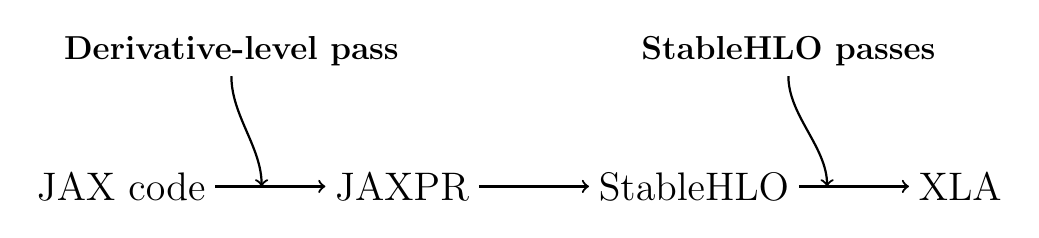
\begin{tikzpicture}[
        node distance=1.4cm,
        every node/.style={font=\Large},
        passlabel/.style={font=\large\bfseries, align=center}
      ]
  
      \node (jax) {JAX code};
      \node[right=of jax] (rewrite) {JAXPR};
      \node[right=of rewrite] (stablehlo) {StableHLO};
      \node[right=of stablehlo] (xla) {XLA};
  
      \draw[->, thick] (jax) -- (rewrite);
      \draw[->, thick] (rewrite) -- (stablehlo);
      \draw[->, thick] (stablehlo) -- (xla);
  
      \node[passlabel, above=1.1cm of jax, xshift=1.4cm] (deriv)
        {Derivative-level pass};
      \draw[->, thick]
        (deriv.south) .. controls +(0,-0.5) and +(0,0.5) .. ($(jax)!0.5!(rewrite)$);
  
      \node[passlabel, above=1.1cm of stablehlo, xshift=1.2cm] (stable)
        {StableHLO passes};
      \draw[->, thick]
        (stable.south) .. controls +(0,-0.5) and +(0,0.5) .. ($(stablehlo)!0.5!(xla)$);
  
    \end{tikzpicture}
    \caption{Compilation pipeline showing where our compiler passes are inserted. The derivative-level pass rewrites the higher-order derivative computation before lowering, while the StableHLO passes optimize the lowered IR before dispatching to XLA.}
    \label{fig:stablehlo-optimization-pipeline}
\end{figure*}


\paragraph{Direct Input-Laplacian Recurrence for Tanh MLPs.}
Our first optimization targets the scalar tanh-MLP Laplacian benchmark.
Rather than lowering a generic higher-order AD expression such as
\texttt{hessian(f)}, repeated \texttt{jvp} applications, or Taylor-mode AD,
we generate code for a direct forward recurrence that computes the
input Laplacian of the network.

For each layer, the ordinary forward pass computes
\[
  z_\ell = a_{\ell-1}W_\ell + b_\ell,
  \qquad
  a_\ell = \tanh(z_\ell).
\]
The optimized recurrence augments this forward pass with two input-derivative
quantities: the Jacobian
\[
  G_\ell = \frac{\partial a_\ell}{\partial x}
\]
and the componentwise input Laplacian
\[
  \lambda_\ell = \Delta a_\ell .
\]
Thus each layer propagates the triple
\[
  (a_\ell, G_\ell, \lambda_\ell),
\]
where \(a_\ell\) is the activation, \(G_\ell\) records first derivatives with
respect to the original input, and \(\lambda_\ell\) records the Laplacian of
each activation component.

The recurrence is initialized by
\[
  a_0 = x,
  \qquad
  G_0 = I,
  \qquad
  \lambda_0 = 0.
\]
For the affine part of layer \(\ell\), derivatives propagate linearly:
\[
  G^z_\ell = G_{\ell-1} W_\ell,
  \qquad
  \lambda^z_\ell = \lambda_{\ell-1} W_\ell .
\]
The tanh nonlinearity is then handled by the chain rule:
\[
  a_\ell = \tanh(z_\ell),
\]
\[
  G_\ell =
    \tanh'(z_\ell) \odot G^z_\ell,
\]
and
\[
  \lambda_\ell =
    \tanh''(z_\ell) \odot
      \|G^z_\ell\|_{\mathrm{row}}^2
    +
    \tanh'(z_\ell) \odot \lambda^z_\ell .
\]
Here \(\|G^z_\ell\|_{\mathrm{row}}^2\) denotes the squared norm of the
input-gradient vector for each activation component. Using $\tanh'(z) = 1 - \tanh^2(z)$ and $\tanh''(z) = -2\tanh(z)(1-\tanh^2(z))$,
the recurrence lowers to ordinary tensor operations such as
\texttt{dot\_general}, \texttt{tanh}, \texttt{multiply}, \texttt{add}, and
\texttt{reduce}.

This computes the same input Laplacian as the corresponding higher-order AD
program, but avoids materializing the full Hessian or constructing a large
nested derivative computation.


\paragraph{Constant Propagation}
Higher-order AD, especially Taylor-mode AD, can introduce scalar coefficient
computations that are independent of the program input. In the StableHLO emitted
by \texttt{jax.experimental.jet}, these appear as constant \texttt{chlo.lgamma}
calls, followed by \texttt{exponential}, \texttt{convert},
\texttt{broadcast\_in\_dim}, and arithmetic operations used to scale Taylor
coefficients. Our constant propagation pass evaluates such scalar and splat
constant expressions before dispatching the program to XLA.

For example, a derivative-generated StableHLO program may contain:
\begin{verbatim}
// Before constant propagation
%cst = stablehlo.constant
       dense<1.00e+01> : tensor<f32>
%0 = chlo.lgamma %cst
     : tensor<f32> -> tensor<f32>
\end{verbatim}

The pass rewrites this to:
\begin{verbatim}
// After constant propagation
%0 = stablehlo.constant
     dense<1.280183e+01> : tensor<f32>
\end{verbatim}

The same pass also folds chains of constant operations. For example, Jet often
emits coefficient-normalization code of the form:
\begin{verbatim}
%cst = stablehlo.constant
       dense<3.00e+00> : tensor<f32>
%0 = chlo.lgamma %cst
     : tensor<f32> -> tensor<f32>
%1 = stablehlo.exponential %0
     : tensor<f32>
%2 = stablehlo.broadcast_in_dim %1,
     dims = []
     : (tensor<f32>)
       -> tensor<256x3xf32>
\end{verbatim}
After constant propagation, the \texttt{lgamma} and \texttt{exponential}
operations are replaced by constants, leaving a simpler StableHLO program with
fewer Taylor-mode bookkeeping operations.

\paragraph{Structural Zero Elimination}
Higher-order AD also introduces tangent, cotangent, or Taylor-coefficient
values that are zero by construction. These zeros can be broadcast, reshaped,
and propagated through arithmetic before later passes remove them. Our
structural zero elimination pass tracks syntactically known zero SSA values in
StableHLO and rewrites operations whose results are also known to be zero.

For example, Jet-generated code often contains broadcasted zero tensors that
are immediately added into a derivative computation:
\begin{verbatim}
// Before structural zero elimination
%z = stablehlo.constant
     dense<0.00e+00> : tensor<f32>
%0 = stablehlo.broadcast_in_dim %z,
     dims = []
     : (tensor<f32>)
       -> tensor<256x3x256xf32>
%1 = stablehlo.add %0, %x
     : tensor<256x3x256xf32>
\end{verbatim}

Since \texttt{\%0} is known to be zero, the addition can be replaced by an alias
to \texttt{\%x}:
\begin{verbatim}
// After structural zero elimination
%1 = %x
\end{verbatim}

\section{Evaluation}
We evaluate the optimization passes on two higher-order differentiation
workloads implemented in JAX: an input-space Laplacian of a scalar MLP and a
Poisson physics-informed neural network (PINN).  In both benchmarks, we compare
three mathematically equivalent ways of computing the required second
derivatives:
\texttt{hessian}, \texttt{jvp\_grad}, and \texttt{jet}.  We do not include the
automatic schedule-selection path in this paper; all reported methods are fixed
source-level AD formulations.

\paragraph{Methods.}
The \texttt{hessian} method computes the dense Hessian of the scalar function
with \texttt{jax.hessian} and takes the trace.  The \texttt{jvp\_grad} method
forms Hessian-vector products by applying \texttt{jax.jvp} to
\texttt{jax.grad}; for each standard basis direction \(e_i\), it computes
\(e_i^\top \nabla^2 f(x)e_i\), then sums over \(i\).  The \texttt{jet} method
uses \texttt{jax.experimental.jet} to propagate second-order Taylor
coefficients along each basis direction and sums the resulting second
directional derivatives.  These methods produce the same mathematical
Laplacian, but they expose different StableHLO programs to the compiler.

\paragraph{Benchmarking protocol.}
For each benchmark and method, the Python benchmark lowers the JAX function to
StableHLO, compiles the original StableHLO through XLA/PJRT, runs untimed
warmup executions, and then records timed executions.  The default timing
configuration uses three warmup runs and thirty measured runs.  To test how the
methods scale with model width, we sweep the hidden dimension
\[
  h \in \{128, 256, 384, 512\}
\]
for both benchmarks while holding the number of layers, input dimension, number
of evaluation points, seed, dtype, and AD method fixed.  We report JIT compile
time and steady-state execution time for the original StableHLO and for the
StableHLO after our optimization-pass pipeline.  The benchmark scripts also
record the backend, output summary, and pass-level compiler statistics.  In the
tables below, the compile-time column reports original StableHLO compile time,
the after-pass compile-time column reports compile time for the transformed
StableHLO, and the runtime columns report average execution time across the
measured runs.

\subsection{MLP Laplacian}
The first benchmark computes the input Laplacian of a scalar fully connected
tanh MLP.  The network has input dimension \(3\), output dimension \(1\), and
\(128\) hidden layers.  We vary the hidden width
\(h \in \{128,256,384,512\}\).  Each hidden layer applies an affine map followed
by \(\tanh\); the final layer is linear.  We initialize weights from a normal
distribution scaled by \(1/\sqrt{\text{fan-in}}\), use zero biases, and store
all parameters in \texttt{float32}.  The benchmark uses seed \(0\).

The input batch contains \(256\) points in \(\mathbb{R}^3\).  In the code, these
points are generated deterministically by linearly spacing
\(256 \times 3\) \texttt{float32} values between \(-1\) and \(1\), then
reshaping them into a \(256 \times 3\) matrix.  For each point \(x\), the task
computes
\[
  \Delta f_\theta(x)
  =
  \operatorname{tr}\left(\nabla_x^2 f_\theta(x)\right),
\]
and the benchmark returns the vector of \(256\) Laplacian values.  This workload
isolates input-derivative computation: the neural network parameters are fixed,
and no outer parameter-gradient computation is performed.

\subsection{Poisson PINN}
The second benchmark evaluates a Poisson PINN residual and differentiates the
loss with respect to network parameters.  The neural network again uses
\(128\) hidden tanh layers, but the input dimension is \(2\) and the output
dimension is \(1\).  We use the same hidden-width sweep
\(h \in \{128,256,384,512\}\), with the same seed-\(0\), \texttt{float32},
fan-in-scaled normal weight initialization and zero-bias initialization.

The PINN defines a trial solution
\[
  u_\theta(x,y) = x(1-x)y(1-y)N_\theta(x,y),
\]
where the multiplicative boundary factor enforces zero boundary values on the
unit square.  Collocation points are a \(16 \times 16\) tensor-product grid,
giving \(256\) points total, with each coordinate linearly spaced from \(0.1\)
to \(0.9\).  At each collocation point, the benchmark computes the residual
\[
  r_\theta(x,y)
  =
  \Delta u_\theta(x,y)
  +
  \sin(\pi x)\sin(\pi y).
\]
The scalar loss is
\[
  \mathcal{L}(\theta)
  =
  \frac{1}{256}\sum_{(x,y)} r_\theta(x,y)^2,
\]
and the benchmarked JAX program returns both
\(\mathcal{L}(\theta)\) and \(\nabla_\theta \mathcal{L}(\theta)\) via
\texttt{jax.value\_and\_grad}.  Thus, unlike the MLP Laplacian benchmark, this
workload nests input-space second derivatives inside an outer reverse-mode
parameter-gradient computation.

\begin{table*}[t]
\centering
\caption{MLP Laplacian results under a hidden-width sweep.  Runtime columns are
average runtime over 30 measured executions.}
\label{tab:mlp-laplacian-results}
\begin{tabular}{clrrrrr}
\toprule
Hidden width & Method & Compile before & Compile after & Runtime before
& Runtime after & Speedup \\
 & & (ms) & (ms) & (ms) & (ms) & \\
\midrule
\multirow{3}{*}{128}
& \texttt{hessian} & 330.9 & 222.0 & 54.3 & 31.0 & 1.75 \\
& \texttt{jvp\_grad} & 286.2 & 222.0 & 54.9 & 30.9 & 1.77 \\
& \texttt{jet} & 404.2 & 254.3 & \textbf{45.1} & \textbf{30.4} & 1.49 \\
\midrule
\multirow{3}{*}{256}
& \texttt{hessian} & 256.5 & 176.9 & 101.6 & 60.0 & 1.69 \\
& \texttt{jvp\_grad} & 240.7 & 176.3 & \textbf{95.4} & 63.9 & 1.49 \\
& \texttt{jet} & 379.0 & 179.4 & 105.4 & \textbf{59.8} & 1.76 \\
\midrule
\multirow{3}{*}{384}
& \texttt{hessian} & 268.5 & 185.5 & 183.0 & 112.2 & 1.63 \\
& \texttt{jvp\_grad} & 237.5 & 183.3 & \textbf{180.4} & \textbf{111.6} & 1.62 \\
& \texttt{jet} & 430.2 & 183.4 & 215.5 & 125.4 & 1.72 \\
\midrule
\multirow{3}{*}{512}
& \texttt{hessian} & 323.3 & 186.2 & 308.4 & 195.3 & 1.58 \\
& \texttt{jvp\_grad} & 238.9 & 176.1 & \textbf{295.3} & \textbf{193.9} & 1.52 \\
& \texttt{jet} & 391.6 & 176.8 & 379.6 & 195.7 & 1.94 \\
\bottomrule
\end{tabular}
\end{table*}

\begin{table*}[t]
\centering
\caption{Poisson PINN results under a hidden-width sweep.  Runtime columns are
average runtime over 30 measured executions.}
\label{tab:pinn-results}
\begin{tabular}{clrrrrr}
\toprule
Hidden width & Method & Compile before & Compile after & Runtime before
& Runtime after & Speedup \\
 & & (ms) & (ms) & (ms) & (ms) & \\
\midrule
\multirow{3}{*}{128}
& \texttt{hessian} & 1770.7 & 859.7 & \textbf{107.9} & \textbf{76.9} & 1.40 \\
& \texttt{jvp\_grad} & 1436.3 & 809.1 & 110.8 & 77.3 & 1.43 \\
& \texttt{jet} & 1599.1 & 823.4 & 128.8 & 77.1 & 1.67 \\
\midrule
\multirow{3}{*}{256}
& \texttt{hessian} & 1727.9 & 1030.0 & 217.3 & 176.3 & 1.23 \\
& \texttt{jvp\_grad} & 1458.8 & 813.2 & \textbf{214.7} & 158.2 & 1.36 \\
& \texttt{jet} & 1602.4 & 763.1 & 252.0 & \textbf{155.5} & 1.62 \\
\midrule
\multirow{3}{*}{384}
& \texttt{hessian} & 1670.4 & 822.4 & 434.5 & \textbf{282.5} & 1.54 \\
& \texttt{jvp\_grad} & 1420.8 & 807.8 & \textbf{413.6} & 283.9 & 1.46 \\
& \texttt{jet} & 1627.7 & 797.3 & 515.9 & 282.9 & 1.82 \\
\midrule
\multirow{3}{*}{512}
& \texttt{hessian} & 1786.3 & 783.6 & 711.0 & \textbf{462.7} & 1.54 \\
& \texttt{jvp\_grad} & 1537.8 & 788.6 & \textbf{704.9} & 465.8 & 1.51 \\
& \texttt{jet} & 1612.7 & 781.5 & 844.6 & 465.4 & 1.82 \\
\bottomrule
\end{tabular}
\end{table*}

\section{Discussion}

\subsection{Compiler Optimization Can Change the Best AD Method}
The results show that choosing an AD method before compiler optimization is not
equivalent to choosing one after optimization.  In the unoptimized StableHLO,
the fastest method depends on the derivative formulation and on the benchmark.
For example, in the MLP Laplacian benchmark, \texttt{jet} is fastest at hidden
width \(128\), but \texttt{jvp\_grad} is fastest for widths \(256\), \(384\),
and \(512\).  In the Poisson PINN benchmark, \texttt{hessian} is fastest at
width \(128\), while \texttt{jvp\_grad} is fastest for the larger widths before
our passes are applied. 

After optimization, the ranking changes in several cases.  For the MLP
Laplacian at width \(256\), the fastest method changes from
\texttt{jvp\_grad} before optimization to \texttt{jet} after optimization.  For
the Poisson PINN, the changes are more pronounced: at width \(256\), the fastest
method changes from \texttt{jvp\_grad} to \texttt{jet}, while at widths \(384\)
and \(512\), it changes from \texttt{jvp\_grad} to \texttt{hessian}.  Thus, the
method that gives the best initial compiler IR is not necessarily the method
that gives the best optimized executable.

This behavior illustrates why higher-order AD performance should be evaluated
jointly with compiler optimization.  A source-level AD transform determines the
initial IR, but the compiler may expose, remove, or replace different parts of
that IR.  In our benchmarks, the direct tanh-MLP Laplacian recurrence removes
much of the structural difference between the original Hessian, JVP-of-gradient,
and Taylor-mode formulations.  As a result, after-pass runtimes are often much
closer to each other than before-pass runtimes, especially in the PINN
benchmark.  The remaining differences then reflect a combination of residual
IR structure, compile decisions, and backend execution effects rather than only
the source-level AD formulation.


\subsection{Limitations and Future Work}
This work is a prototype evaluation of compiler optimizations for higher-order
AD, and its scope is intentionally narrow.  The direct Laplacian recurrence is
specialized to scalar tanh MLPs with affine layers, and the evaluation fixes the
input dimension, batch size, number of layers, dtype, and random seed while
sweeping only hidden width.  The Poisson PINN benchmark is more representative
of scientific machine learning because it nests input-space second derivatives
inside an outer parameter-gradient computation, but it is still a single PDE,
single network family, and single collocation-grid shape.  We also evaluate a
single backend configuration; GPU and TPU backends may expose different
tradeoffs between larger derivative IR, backend fusion, memory traffic, and
compile time.

Our StableHLO passes are also conservative.  Constant propagation and
structural zero elimination target patterns that appear in the generated IR for
the benchmarks studied here, and the direct recurrence relies on recognizing a
high-level mathematical structure before lowering.  We do not yet provide a
general optimizer for arbitrary higher-order derivative programs, nor do we
prove equivalence for every possible StableHLO rewrite.  In particular, broader
support for other activations, vector-valued outputs, convolutional networks,
non-MLP PDE solvers, and mixed precision would require additional rewrite rules
and validation.

Future work should extend the pass pipeline in three directions.  First, the
compiler should exploit higher-order derivative identities such as mixed-partial
symmetry, Hessian sparsity, and diagonal-only access patterns.  These identities
could enable common subexpression elimination across derivative subgraphs and
kernel rewrites that avoid forming unused tensor entries.  Second, the current
benchmark suite should be expanded to include additional PDEs, larger input
dimensions, hardware backends, and end-to-end training loops.  Third, the passes
should be integrated more tightly with the JAX/StableHLO lowering path so that
the optimization opportunities are available during normal compilation rather
than through an offline experimental pipeline.

\subsection{Related Work}
Automatic differentiation systems expose derivatives through a range of program
transformation mechanisms.  JAX provides composable transformations such as
\texttt{grad}, \texttt{jvp}, and \texttt{hessian} over NumPy-style programs
\cite{bradbury2018jax}, while PyTorch popularized imperative tensor programs
with high-performance reverse-mode AD for deep learning
\cite{paszke2019pytorch}.  Classical AD treatments describe the algorithmic
foundations of forward, reverse, and higher-order modes
\cite{griewank2008evaluating}.  Taylor-mode AD computes higher-order
derivatives by propagating truncated Taylor coefficients; JAX Jet implements
this idea for JAX programs and avoids some redundant work that arises from
naively composing first-order transformations \cite{bettencourt2019taylor}.
Our evaluation compares Jet against two nested first-order formulations after
lowering to StableHLO, emphasizing that their relative performance depends on
the downstream compiler as well as on the source-level AD algorithm.

Several systems move AD into the compiler.  Enzyme is a high-performance
automatic differentiation compiler plugin for LLVM that differentiates optimized
LLVM IR and targets programs written in languages that lower to LLVM
\cite{moses2020enzyme}.  Later Enzyme work extends this compiler-based approach
to reverse-mode AD for GPU kernels and multiple parallel programming paradigms
\cite{moses2021reverse,moses2022scalable}.  Enzyme is complementary to this
paper: it synthesizes derivative programs at the compiler IR level, while our
prototype starts from derivative programs already produced by JAX and optimizes
the StableHLO tensor IR before XLA compilation.

Compiler optimization for tensor programs is also closely related.  MLIR
provides the extensible compiler infrastructure underlying many domain-specific
IRs, including tensor compiler pipelines \cite{lattner2021mlir}.  TASO shows
that tensor computation graphs can be optimized through automatically generated
graph substitutions \cite{jia2019taso}.  Most closely related to this work,
Sathia et al.\ study compiler optimizations for higher-order AD in StableHLO and
argue that derivative-generated tensor programs contain exploitable structure
such as constants, zeros, symmetry, and sparse access patterns
\cite{sathia2025compiler}.  Our paper follows this compiler-oriented view, but
adds a more detailed evaluation across both standalone MLP Laplacians and a
Poisson PINN workload.  PINNs use neural networks to represent PDE solutions and
rely on differentiating network outputs with respect to physical coordinates
\cite{raissi2019physics}; this makes them a natural setting for testing whether
compiler optimizations improve second-order AD in scientific machine learning.

\section{Conclusion}
Higher-order AD programs are not only mathematical derivative computations; they
are also compiler inputs.  We showed that three equivalent JAX formulations for
Laplacian computations, \texttt{hessian}, \texttt{jvp\_grad}, and
\texttt{jet}, lower to different StableHLO programs and can respond differently
to compiler optimization.  A small optimization pipeline for tanh-MLP
Laplacians and derivative-generated StableHLO reduces both compile time and
steady-state runtime on MLP Laplacian and Poisson PINN benchmarks.

The main empirical lesson is that the best AD method can change after compiler
optimization.  In several settings, the formulation with the fastest original
runtime is not the one with the fastest optimized runtime.  This suggests that
higher-order AD systems should not treat derivative generation and compiler
optimization as separate concerns.  Instead, AD methods should be evaluated by
the optimized executable they produce, and compilers should expose passes that
recognize the structure introduced by higher-order differentiation.

\bibliography{example_paper}
\bibliographystyle{icml2025}


\end{document}


% This document was modified from the file originally made available by
% Pat Langley and Andrea Danyluk for ICML-2K. This version was created
% by Iain Murray in 2018, and modified by Alexandre Bouchard in
% 2019 and 2021 and by Csaba Szepesvari, Gang Niu and Sivan Sabato in 2022.
% Modified again in 2023 and 2024 by Sivan Sabato and Jonathan Scarlett.
% Previous contributors include Dan Roy, Lise Getoor and Tobias
% Scheffer, which was slightly modified from the 2010 version by
% Thorsten Joachims & Johannes Fuernkranz, slightly modified from the
% 2009 version by Kiri Wagstaff and Sam Roweis's 2008 version, which is
% slightly modified from Prasad Tadepalli's 2007 version which is a
% lightly changed version of the previous year's version by Andrew
% Moore, which was in turn edited from those of Kristian Kersting and
% Codrina Lauth. Alex Smola contributed to the algorithmic style files.
